\documentclass{article}
\usepackage[utf8]{inputenc}
\usepackage[spanish]{babel}
\usepackage{listings}
\usepackage{graphicx}
\usepackage{geometry}
\graphicspath{ {images/} }
\usepackage{cite}

\geometry{
textheight=23cm
}
\begin{document}

\begin{titlepage}
    \begin{center}
        \vspace*{0cm}
            
        \large
        \textbf{ARTIC WOLF: SAVING THE FAMILY}
            
        \vfill
            
        \vspace{0.8cm}
            
        \textbf{David Agudelo Ochoa}
        
        \vspace{5mm}
        
        \textbf{Erika Dayana León Quiroga}
            
        \vfill
            
        \vspace{0.8cm}
            
        \Large
        Universidad de Antioquia\\
        Despartamento de Ingeniería Electrónica y Telecomunicaciones\\
        Informática II\\
        Medellín-Antioquia\\
        Abril de 2021
            
    \end{center}
\end{titlepage}

\tableofcontents
\newpage
\section{Sección introductoria.}
En este informe veremos el desarrollo del proyecto final de la materia Informática II, el cual será un juego llamado Gartic Wolf: Saving the family. Dentro de las secciones veremos listas de tareas hechas para organizar mejor el trabajo a realizar, actualizaciones y problemas del código del programa.

\section{Lista de tareas.}
\begin{itemize}
    \item Jueves 7 de Abril:
    \begin{itemize}
        \item Crear proyecto Qt
        \item Crear la clase ObjetoAnimado y las que heredarán de ella.
        \item Objeto animado: Atributos y métodos.
        \item Método StringPath.
        \item Probar método animar.
        \item Instalar librería QMediaPlayer (para sonidos del juego.)
        
    \end{itemize}
    \item Viernes 8 de Abril:
    \begin{itemize}
        \item Agregar atributos y constructor de las clases que heredan de Objeto animado, como héroe, enemigo, proyectil, reloj.
        \item Creación y animación del escenario y el héroe.
        \item Pruebas de la animación.
    
    \end{itemize}
    
    \item Sábado 9 de Abril:
    \begin{itemize}
        \item Agregar métodos de las clases que heredan de Objeto animado, como héroe, enemigo, proyectil, reloj.
        \item Método de proyectil que mueve y verifica la colisión con otros objetos del mismo.
        \item Agregar el método que creará el nivel uno.
        
    
    \end{itemize}
\end{itemize}

\section{Desarrollo del proyecto.}
Para el desarrollo del proyecto Artic Wolf: Saving the Family, se tuvo en cuenta el informe de Clases que se realizó previamente con la intención de tener un plan de organización de las clases que serían necesarias para el funcionamiento del juego que se tiene planeado. En este informe de clases encontramos la descripción nivel por nivel del juego y la descripción clase por clase del mismo. A continuación veremos los cambios que se le realizaron a las clases que se tenían pensadas a la hora de materializar estas ideas en código.

En los días \textbf{Jueves 7 y Viernes 8 de abril} se comenzó por crear el proyecto con la clase padre Objeto animado con sus respectivos atributos y métodos, y sus clases hijas Heroe, Enemigo, Proyectil y Reloj.
En la clase objeto animado se realizaron varios cambios con respecto a lo planeado en el informe de clases. Esto porque a medida que se va escribiendo el código se encuentran formas más efectivas de realizar ciertas tareas que las que ya se tenían planeadas. Sin embargo, el uso del informe de Clases es fundamental para la asignación de tareas y la realización del avance del proyecto.

\newpage
\begin{figure}[h]
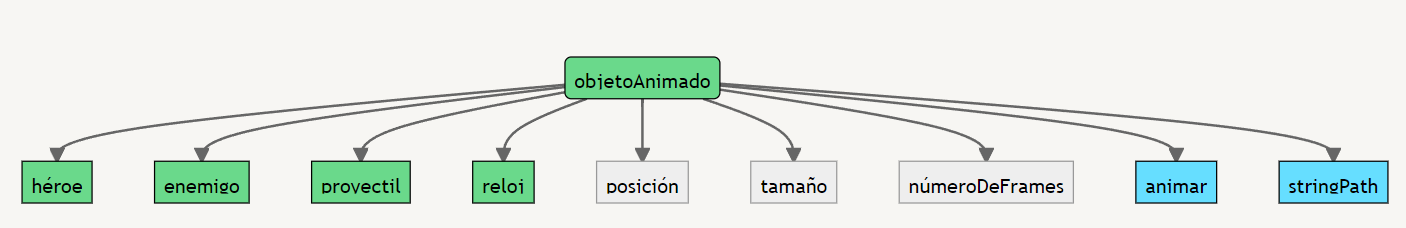
\includegraphics[scale=0.5]{Images/ObjetoAnimado.png}
\centering
\caption{Clase ObjetoAnimado que se tenía pensada construir.}
\label{fig:objetoAnimado}
\end{figure}

\begin{figure}[h]
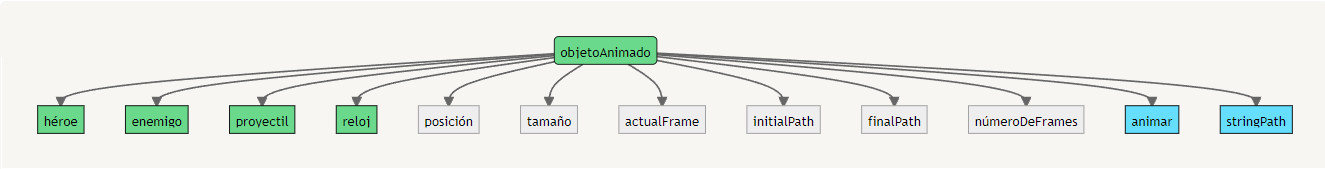
\includegraphics[scale=0.6]{Images/newObjetoanimado.png}
\centering
\caption{Clase ObjetoAnimado construida.}
\label{fig:newobjetoAnimado}
\end{figure}

Con los cambios realizados en la clase objeto animado se logró obtener el movimiento esperado en los objetos que se muestran en la escena, esto con ayuda del método animar y stringPath los cuales siguen cumpliendo las mismas funciones que se les asignaron en la parte de planeación del proyecto. El método stringPath recibe el número de la imagen de la cuál se requiere su path y luego lo retorna. La función animar utiliza el método anterior para conocer el camino a la imagen y haciendo uso de actualFrame como parámetro del método stringPath logra ir cambiando el frame de tal forma que cuando sea llamada, estos varíen y den la impresión de movimiento.

\begin{figure}[h]
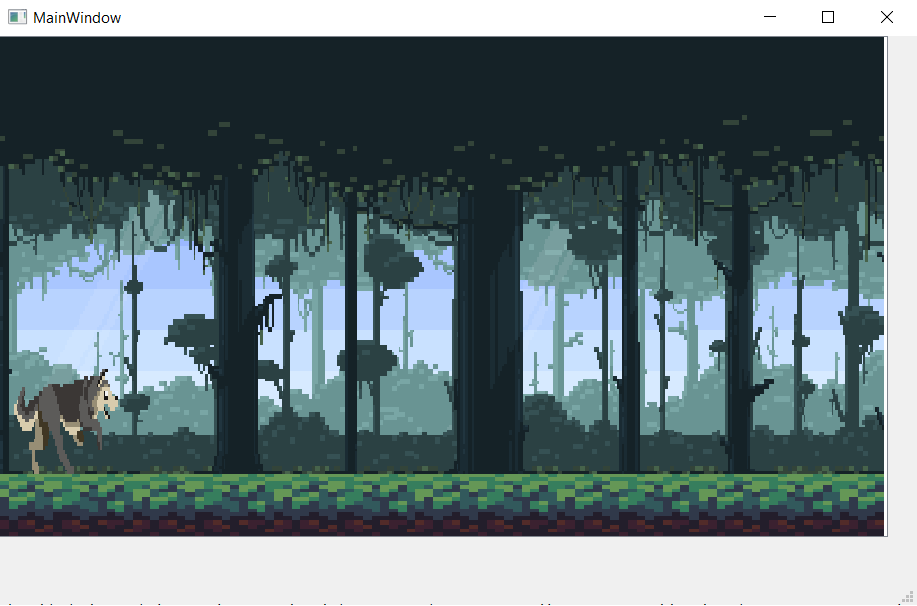
\includegraphics[scale=0.6]{Images/animaciones.png}
\centering
\caption{Pantalla de prueba con el héroe y el fondo animados.}
\label{fig:animacion}
\end{figure}

El \textbf{Sábado 9 de abril} se empezó con la creación de la clase padre Nivel y sus clases hijas nivel1 y nivel2 como se planeó en el informe de Clases. Estas clases se utilizarían para armar el nivel correspondiente en cada clase.

\newpage
\begin{figure}[h]
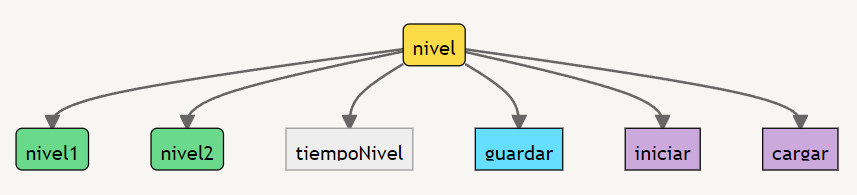
\includegraphics[scale=0.6]{Images/niveles.png}
\centering
\caption{Clase nivel planeada en el informe de clases.}
\label{fig:niveles}
\end{figure}

Sin embargo, nos dimos cuenta que la función que le otorgamos a estas clases en la planeación podría ser reemplazada por un método en el MainWindow que realice la misma función, en este método se agregarían todos los objetos necesarios para crear el nivel correspondiente.



Ir mostrando el avance en imágenes
Las clases niveles serán reemplazadas por métodos de la clase mainwindow

    




\section{Conclusiones.}
    \begin{itemize}
        \item
    \end{itemize}

\end{document}
